\documentclass[12pt,a4paper]{article}
\usepackage[utf8]{inputenc}
\usepackage[english]{babel}
\usepackage{graphicx}
\usepackage{hyperref}
\usepackage{listings}
\usepackage{xcolor}
\usepackage{geometry}
\usepackage{fancyhdr}
\usepackage{amsmath}
\usepackage{amssymb}
\usepackage{multicol}

\geometry{margin=2.5cm}
\setlength{\headheight}{14.5pt}

\lstset{
    basicstyle=\ttfamily\footnotesize,
    keywordstyle=\color{blue}\bfseries,
    commentstyle=\color{green!60!black}\itshape,
    stringstyle=\color{red!80!black},
    identifierstyle=\color{black},
    numberstyle=\tiny\color{gray},
    emphstyle=\color{orange},
    showstringspaces=false,
    breaklines=true,
    frame=single,
    frameround=tttt,
    backgroundcolor=\color{gray!5},
    rulecolor=\color{gray!40},
    numbers=none,
    numbersep=8pt,
    captionpos=b,
    tabsize=4,
    xleftmargin=10pt,
    xrightmargin=5pt,
    framexleftmargin=5pt
}

% Definition for DOT language (Graphviz)
\lstdefinelanguage{DOT}{
    keywords={digraph, graph, node, edge, subgraph},
    sensitive=true,
    comment=[l]{//},
    morecomment=[s]{/*}{*/},
    morestring=[b]",
    keywordstyle=\color{blue}\bfseries,
    commentstyle=\color{green!60!black}\itshape,
    stringstyle=\color{red!80!black}
}

% Definition for JSON
\lstdefinelanguage{json}{
    basicstyle=\ttfamily\footnotesize,
    numbers=none,
    numberstyle=\tiny\color{gray},
    stepnumber=1,
    numbersep=8pt,
    showstringspaces=false,
    breaklines=true,
    frame=single,
    backgroundcolor=\color{gray!5},
    string=[s]{"}{"},
    stringstyle=\color{red!80!black},
    comment=[l]{:},
    commentstyle=\color{black},
    morecomment=[l]{//},
    morecomment=[s]{/*}{*/},
    literate=
     *{0}{{{\color{orange}0}}}{1}
      {1}{{{\color{orange}1}}}{1}
      {2}{{{\color{orange}2}}}{1}
      {3}{{{\color{orange}3}}}{1}
      {4}{{{\color{orange}4}}}{1}
      {5}{{{\color{orange}5}}}{1}
      {6}{{{\color{orange}6}}}{1}
      {7}{{{\color{orange}7}}}{1}
      {8}{{{\color{orange}8}}}{1}
      {9}{{{\color{orange}9}}}{1}
      {:}{{{\color{blue}{:}}}}{1}
      {,}{{{\color{blue}{,}}}}{1}
      {\{}{{{\color{purple}{\{}}}}{1}
      {\}}{{{\color{purple}{\}}}}}{1}
      {[}{{{\color{purple}{[}}}}{1}
      {]}{{{\color{purple}{]}}}}{1}
      {true}{{{\color{blue!80!black}true}}}{4}
      {false}{{{\color{blue!80!black}false}}}{5}
      {null}{{{\color{blue!80!black}null}}}{4}
}

\pagestyle{fancy}
\fancyhf{}
\rhead{peshmind}
\lhead{}
\rfoot{Page \thepage}

\title{

\includegraphics[width=0.3\textwidth]{img/logo.png} \\
\vspace{1cm}
\large \textcolor{red}{P}rolog-based \textcolor{red}{E}ngine for \textcolor{red}{S}ystem \& \textcolor{red}{H}ost \textcolor{red}{M}anagement and \textcolor{red}{In}ference \textcolor{red}{D}aemon \\
\vspace{1cm}
}
\author{Mirko Mariotti}
\date{March 2026}

\begin{document}

\maketitle
\thispagestyle{empty}

\newpage
\tableofcontents
\newpage

\section{Introduction}

peshmind is a system for discovering and analyzing LAN network topology based exclusively
on MAC addresses observed by network switches.
The system combines a Go-written CLI application with a Prolog engine to identify 
network connections, internal/access switches, and potential "ghost switches" (unlisted switches)
present in the network infrastructure.

\subsection{Motivation and Objectives}

In complex large-scale networks, physical topology documentation often becomes obsolete 
or incomplete. peshmind addresses this problem by providing an automated system that:

\begin{itemize}
    \item Reconstructs network topology by analyzing only switch MAC tables
    \item Automatically identifies unlisted switches ("ghost switches"), enabling the discovery of anomalies and unauthorized devices
    \item Distinguishes between core/distribution switches and access switches
    \item Provides graphical visualizations of the inferred topology
\end{itemize}

\section{System Architecture}

\subsection{Main Components}

The peshmind system consists of three main components that interact with each other:

\subsubsection{Go CLI Application}

The CLI application \textbf{peshmind}, developed in Go, coordinates all system operations, including the
other two components. Its subcommands, implemented with the Cobra framework, manage the following functionalities:

\begin{itemize}
    \item Automatic retrieval of MAC tables from physical switches
    \item Conversion of data into Prolog facts
    \item Starting and managing the Prolog engine
    \item Querying the inference system
    \item Generation of DOT visualizations
    \item Simulation of network topologies
\end{itemize}

\subsubsection{Prolog Inference Engine}

The Prolog engine (SWI-Prolog) analyzes facts related to MAC addresses and infers the network topology through logical rules. It uses the Pengines library to expose a RESTful HTTP endpoint.

\subsubsection{Knowledge Base}

The knowledge base stores switch and MAC address data in the form of Prolog facts:

\begin{itemize}
    \item \texttt{switch(MacAddr)} - Declares the existence of a switch
    \item \texttt{switchname(MacAddr, Name)} - Associates a MAC with a name
    \item \texttt{seen(SwitchMac, DeviceMac, Port)} - Records MACs seen on specific ports
\end{itemize}

\subsection{Two Possible Workflows}

The system supports two main workflows: analysis of an existing network and 
simulation of network topologies. The second is particularly useful for testing and validating Prolog
inference rules before applying them to real data. \\
Broadly speaking, the workflows follow the steps described below; the topic will be explored in detail in subsequent
sections with practical examples and technical details.

\begin{multicols}{2}
        \textbf{Existing Network Analysis}
        \begin{enumerate}
            \item Switch configuration in \texttt{peshmind.json}
            \item MAC table acquisition via SSH or telnet
            \item Data conversion into Prolog facts
            \item KB loading and inference
            \item Query and visualization of results
        \end{enumerate}
\columnbreak
        \textbf{Network Topology Simulation}
        \begin{enumerate}
            \item Creation of DOT file with desired topology
            \item Simulation execution to generate Prolog facts
            \item KB loading and inference
            \item Query and visualization of results
            \item Iteration to test different configurations
        \end{enumerate}
\end{multicols}

\subsection{Code Structure}

The project sources are organized in the following structure:

\begin{verbatim}
peshmind/
|-- main.go              # Application entry point
|-- cmd/                 # Cobra commands
|   |-- root.go         # Root command
|   |-- list.go         # List configured switches
|   |-- update.go       # Update switch data
|   |-- serve.go        # Start Prolog engine
|   |-- query.go        # Query the engine
|   |-- dot.go          # Generate DOT file
|   +-- simulate.go     # Simulate topologies
|-- pkg/peshmind/        # Business logic
|   |-- peshmind.go     # Configuration
|   |-- switch.go       # Switch management
|   |-- spawn.go        # Prolog engine startup
|   +-- simulate.go     # Simulation logic
+-- kbpool/              # Prolog knowledge base
    |-- rules.pl        # Inference rules
    |-- server.pl       # Pengines HTTP server
    +-- createkb.sh     # KB creation script
\end{verbatim}
\subsection{Technologies Used}

\subsubsection{Go}

The Go language was chosen for the CLI application as it offers excellent performance,
 allows static compilation with generation of a single easily deployable binary, 
 provides excellent support for concurrent programming, and makes available a rich
  ecosystem of ready-to-use libraries. \\
The Go libraries that were used include:
\begin{itemize}
    \item \textbf{Cobra}: CLI framework for commands and flags
    \item \textbf{Pengine Client}: Go client to query Pengines
    \item \textbf{go-graphviz}: Parsing and generation of DOT graphs
    \item \textbf{golang.org/x/term}: Secure password input
\end{itemize}
\subsubsection{SWI-Prolog}

SWI-Prolog provides the inference engine thanks to a powerful logical inference system, the 
Pengines library for exposing HTTP APIs, a declarative syntax particularly suited to 
defining complex rules, and excellent performance even on large knowledge bases.

\section{Installation}
\subsection{Prerequisites}

To compile and run peshmind, the following software is required

\begin{itemize}
    \item Git (to clone the repository)
    \item Go 1.20 or higher (to compile the CLI application)
    \item SWI-Prolog 8.0 or higher (for the inference engine)
    \item Graphviz (for visualization generation)
\end{itemize}

\subsection{Installation}

The application can be downloaded from the project's GitHub repository \\

\begin{lstlisting} 
    git clone https://github.com/mmirko/peshmind.git
\end{lstlisting}

After cloning the repository, you can compile the CLI application with the command: \\
\begin{lstlisting}
    cd peshmind
    go build -o peshmind main.go
\end{lstlisting}

The compiled binary will be available in the current directory and can be executed from the terminal.
Alternatively, you can copy the binary to a directory in your PATH to make it globally accessible. \\

In this case, you need to ensure you keep the \texttt{kbpool} directory and the Prolog files inside it, as they
are necessary for the correct functioning of the system.

\section{Usage}
\subsection{General CLI Commands}

Most of peshmind's CLI commands can be used both for real network analysis and for 
topology simulation, as they operate on the Prolog facts generated by both modes. \\
For correct command execution, in either mode, the following are required: the \texttt{peshmind.json} configuration file 
and the Prolog facts in the \texttt{kbpool} directory (generated by \texttt{update} or \texttt{simulate} depending on the mode)
which also contains the inference rules (\texttt{rules.pl}) and the Pengines server (\texttt{server.pl}).

\subsubsection{List}

The \texttt{list} command displays all configured switches with their details:

\begin{lstlisting}[language=bash]
peshmind list
\end{lstlisting}

\subsubsection{Serve}

The \texttt{serve} command starts the Prolog engine with HTTP endpoint:

\begin{lstlisting}[language=bash]
peshmind serve --kbpool kbpool
\end{lstlisting}

Once started, the engine is ready to receive queries and respond with logical inference results.
Technically, this command launches and keeps active a Prolog process that loads facts and rules from the
\texttt{kbpool} directory and exposes a RESTful HTTP endpoint for querying. The process remains active until it is
interrupted manually with CTRL+C or with a process termination command.

\subsubsection{Query}

The \texttt{query} command allows you to query the Prolog engine:

\begin{lstlisting}[language=bash]
# Find all switches
peshmind query "switch(X)"

# Find directly connected switches
peshmind query "directn(X,Y)"

# Identify ghost switches
peshmind query "ghostn(X,Y)"
\end{lstlisting}

In this case, the command sends the query to the peshmind instance running the \texttt{serve} subcommand and receives
the results, which are then formatted and printed to the terminal. \\
The two subcommands \texttt{query} and \texttt{serve} are designed to be used together, 
where \texttt{serve} keeps the Prolog engine active and \texttt{query} sends inference requests. \\
For details on the implemented inference rules, refer to section \ref{sec:inference}.

\subsubsection{Dot}

The \texttt{dot} command generates a DOT file that represents the inferred topology. This file can be visualized 
with Graphviz tools (dot, fdp, neato, etc.) to obtain a graphical representation of the network: \\

\begin{lstlisting}[language=bash]
peshmind dot > network.dot
dot -Tpng network.dot -o network.png
\end{lstlisting}

The generated DOT file includes:
\begin{itemize}
    \item Cluster for each switch with its ports
    \item Physical connections between ports
    \item Ghost switches highlighted with different style
    \item Color coding for better readability
\end{itemize}

\subsection{Commands for Real Network Analysis}

\subsubsection{Update}

The \texttt{update} command retrieves MAC tables from switches: \\

\begin{lstlisting}[language=bash]
# Update a specific switch
peshmind update --switch switch-01

# Update all switches
peshmind update --switch all
\end{lstlisting}

This command:
\begin{enumerate}
    \item Connects to the switch via SSH or telnet using credentials provided in the configuration file
    \item Processes a command template specific to the switch model and, using expect, interacts with the switch shell to execute the commands necessary to obtain the MAC table
    \item Parses the output with regular expressions
    \item Generates Prolog facts in \texttt{seen/3} format
    \item Saves the file in the \texttt{kbpool} directory
\end{enumerate}

\subsection{Commands for Topology Simulation}

\subsubsection{Simulate}

The \texttt{simulate} command allows you to test topologies:

\begin{lstlisting}[language=bash]
peshmind simulate --simname topology.dot \
    --emit-dot output.dot \
    --output facts.pl
\end{lstlisting}

Like the \texttt{update} command, it also generates Prolog facts, but instead of connecting to real switches,
it generates facts programmatically from a DOT file describing the desired topology. It supports
special attributes to identify ghost switches, specify MAC addresses and connection ports. Details on the
DOT file structure and supported attributes are provided in section \ref{sec:conf}.

\section{Logical Inference with Prolog}
\label{sec:inference}

The heart of the system is the Prolog inference engine, which uses the generated facts to deduce the network topology.
This section describes the main inference rules implemented in Prolog.

\subsection{Predicate far/2}

Two switches are "far" if they are connected to a third switch on the same port:

\begin{lstlisting}[language=Prolog]
far(X,Y) :- 
    seen(X,K,MIDPORTX), 
    seen(Y,K,MIDPORTY),
    seen(X,Y,PORTX),
    seen(Y,X,PORTY),
    switch(K), switch(X), switch(Y), 
    X \= Y, Y \= K, X \= K, 
    PORTX == MIDPORTX,
    PORTY == MIDPORTY.
\end{lstlisting}

This predicate identifies the presence of an intermediate switch between two switches.

\subsection{Predicate direct/2}

Two switches are directly connected if they are not far:

\begin{lstlisting}[language=Prolog]
direct(X,Y) :- \+ far(X,Y).
\end{lstlisting}

\subsection{Predicate directp/4}

Direct connection with port information:

\begin{lstlisting}[language=Prolog]
directp(X,Y,PORTX,PORTY) :- 
    seen(X,Y,PORTX),
    seen(Y,X,PORTY),
    \+ far(X,Y).
\end{lstlisting}

\subsection{Predicate ghost/2}

Identifies ghost switches between two directly connected switches:

\begin{lstlisting}[language=Prolog]
ghost(X,Y) :- 
    directp(X,Y,PORTX,PORTY),
    seen(X,Z,PORTX),
    seen(Y,Z,PORTY),
    \+ switch(Z).
\end{lstlisting}

If two switches see the same MAC (non-switch) on the interconnection ports, a ghost switch exists.

\subsection{Predicate internalswitch/1}

Identifies internal switches (core/distribution):

\begin{lstlisting}[language=Prolog]
internalswitch(X) :- 
    seen(X,Y,PORT1),
    seen(X,Z,PORT2),
    switch(X), switch(Y), switch(Z), 
    X \= Y, X \= Z, Y \= Z,
    PORT1 \= PORT2.
\end{lstlisting}

A switch is internal if it is connected to at least two different switches.

\subsection{Predicate edgeswitch/1}

Identifies access switches:

\begin{lstlisting}[language=Prolog]
edgeswitch(X) :- switch(X), \+ internalswitch(X).
\end{lstlisting}

\section{Configuration Details}
\label{sec:conf}

\subsection{Configuration File}

The \texttt{peshmind.json} file defines switches and system parameters in both modes 
(analysis and simulation). Here is a configuration example:

\begin{lstlisting}[language=json]
{
  "debug": true,
  "endpoint": "http://localhost:3030/pengine",
  "switches": {
    "switch-01": {
      "name": "switch-01",
      "mac": "aabbccddeeff",
      "description": "Core Switch Floor 1",
      "ip": "192.168.1.10",
      "username": "admin",
      "password": "ask",
      "model": "HP-Aruba",
      "port": 48,
      "extraports": [],
      "data": ""
    }
  }
}
\end{lstlisting}

\begin{itemize}
    \item \textbf{debug}: Enables verbose output
    \item \textbf{endpoint}: URL of the Pengines HTTP endpoint
    \item \textbf{switches}: Dictionary of switch configurations
    \begin{itemize}
        \item \textbf{name}: Unique switch identifier
        \item \textbf{mac}: Switch MAC address (without separators)
        \item \textbf{description}: Human-readable description
        \item \textbf{ip}: Management IP address
        \item \textbf{username}: SSH/telnet username
        \item \textbf{password}: SSH/telnet password (use "ask" for interactive input)
        \item \textbf{model}: Switch model (for command templates)
        \item \textbf{port}: Number of physical ports
        \item \textbf{extraports}: Additional ports (e.g. trunk, uplink, etc.)
    \end{itemize}
\end{itemize}

\subsection{Existing Network Analysis Mode}
To analyze an existing network, you only need to correctly configure the \texttt{peshmind.json} file 
with access information for each managed switch.

\subsection{Simulation Mode}

In the case of simulation, in addition to the configuration, it is necessary to create a DOT file describing the desired
network topology. The DOT file must follow a specific structure to be correctly analyzed by the simulation
system.
The simulation mode allows testing topologies using DOT files. The system:

\begin{enumerate}
    \item Analyzes the DOT graph using the \texttt{go-graphviz} library
    \item Identifies switch nodes (normal and ghost)
    \item Extracts connections from graph edges
    \item Generates fictitious MAC addresses for end-node devices
    \item Produces equivalent Prolog facts
    \item Supports the following special attributes that can be added to nodes:
    \begin{itemize}
        \item \texttt{ghost="true"} - Specifies that the node is a ghost switch
        \item \texttt{mac="..."} - Specifies MAC for ghost switch
        \item \texttt{port="N"} - Specifies connection port
        \item \texttt{ports="N"} - Number of ports for ghost switch
    \end{itemize}
\end{enumerate}

An example DOT file for simulation is shown in section \ref{sec:examples}.

\section{Usage Examples}
\label{sec:examples}

\subsection{Simulation of a 3-Switch Network}

Suppose we want to simulate a network with 3 switches. The DOT file, let's call it \texttt{topology3.dot}, could be as follows: \\
\begin{lstlisting}[language=DOT]
    digraph dsgraph {
	node [label="\N"];
	"switch-0-1";
	"switch-0-2";
	"switch-3-5";
	"switch-0-1" -> "switch-0-2" [port = 24]; 
	"switch-0-2" -> "switch-0-1" [port = 24];
	"switch-0-1" -> "switch-3-5" [port = 23];
	"switch-3-5" -> "switch-0-1" [port = 23];
}
\end{lstlisting}

In this example, we have three switches (switch-0-1, switch-0-2, switch-3-5) of which one is central (switch-0-1) connected to the 
other two. \\

By executing the simulation command, we obtain the output shown below, which includes switch identification,
connection ports, and generation of corresponding Prolog facts. \\
\begin{lstlisting}[language=bash]
# Topology simulation from DOT file
% peshmind simulate --config peshmind.json -d simout.dot -o kbpool -s topology3.dot --sim-generate-percentage 30
# Debug output:
Found switch in graph: switch-0-1
Switch switch-0-1 has 24 ports and extra ports: []
Found switch in graph: switch-0-2
Switch switch-0-2 has 24 ports and extra ports: []
Found switch in graph: switch-3-5
Switch switch-3-5 has 24 ports and extra ports: []
Edge name: %3 from switch-0-1 to switch-0-2 port: 24
Edge name: %7 from switch-0-1 to switch-3-5 port: 23
Edge name: %1 from switch-0-2 to switch-0-1 port: 24
Edge name: %5 from switch-3-5 to switch-0-1 port: 23
Switch ports mapping: map[switch-0-1:map[23:switch-3-5 24:switch-0-2] switch-0-2:map[24:switch-0-1] switch-3-5:map[23:switch-0-1]]
DOT file written to simout.dot
Output file written to kbpool/switch-0-1.pl
Output file written to kbpool/switch-0-2.pl
Output file written to kbpool/switch-3-5.pl
\end{lstlisting}

The generated DOT file (\texttt{simout.dot}), in figure \ref{fig:simout3}, represents the simulated topology, while the Prolog files in the
\texttt{kbpool} directory contain the facts generated for each switch, ready to be loaded into the inference engine. \\

\begin{figure}[ht]
    \centering
    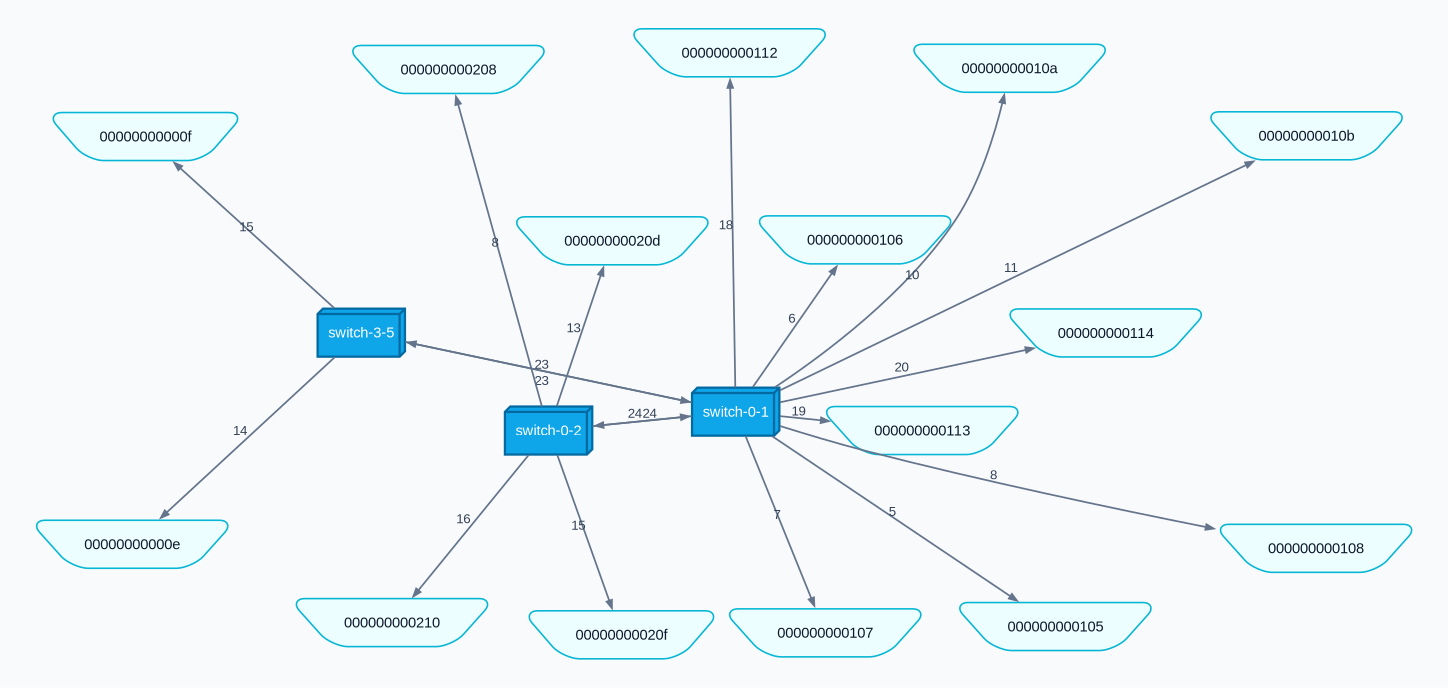
\includegraphics[width=.9\textwidth]{img/simout3.png}
    \caption{Visualization of the simulated topology with 3 switches}
    \label{fig:simout3}
\end{figure}

The files generated by the simulator can be used in analysis mode. The \texttt{serve} command loads the facts
into the knowledge base and starts the inference engine, allowing queries to be executed to identify the topology. \\

\begin{lstlisting}[language=bash]
# Starting the Prolog engine with simulated facts
peshmind serve --kbpool kbpool
\end{lstlisting}

Once the engine is started, you can execute queries like those shown below. \\

\begin{lstlisting}[language=bash]
# Query to identify edge switches (edgeswitch)
% peshmind query "edgeswitchpn(X,N)"
# Output:
&{edgeswitchpn [switch-0-2 24]}
&{edgeswitchpn [switch-0-2 24]}
&{edgeswitchpn [switch-3-5 23]}
&{edgeswitchpn [switch-3-5 23]}

# Query to identify directly connected switches
% peshmind query "directpn(X,Y,PORTX,PORTY)"
# Output:
&{directpn [switch-0-1 switch-0-2 24 24]}
&{directpn [switch-0-1 switch-3-5 23 23]}
&{directpn [switch-0-2 switch-0-1 24 24]}
&{directpn [switch-3-5 switch-0-1 23 23]}
\end{lstlisting}

Finally, it is possible to generate a graphical visualization,
shown in figure \ref{fig:inferred3},
of the inferred topology using the \texttt{dot} command. \\
\begin{lstlisting}[language=bash]
# DOT file generation from inferred topology
peshmind dot > inferred_topology.dot
dot -Tpng inferred_topology.dot -o inferred_topology.png
\end{lstlisting}

\begin{figure}[ht]
    \centering
    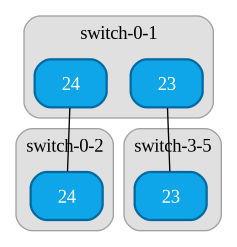
\includegraphics[width=.3\textwidth]{img/inferred3.png}
    \caption{Visualization of the inferred topology with 3 switches}
    \label{fig:inferred3}
\end{figure}

As can be seen, the inferred topology corresponds exactly to the simulated one, with switch-0-1 identified as a core
switch and switch-0-2 and switch-3-5 identified as access switches, with interconnection ports correctly highlighted. \\

\subsection{Simulation of a 6-Switch Star}

Starting from a star topology with 6 switches as shown in the \texttt{topology6star.dot} file below, it is 
possible to run the simulation and inference to identify the topology. \\

\begin{lstlisting}[language=DOT]
digraph dsgraph {
	node [label="\N"];
	"switch-0-1";
	"switch-0-2";
	"switch-0-3";
	"switch-3-5";
	"switch-3-30";
	"switch-3-31"; 
	"switch-3-5" -> "switch-0-2" [port = 22]; 
	"switch-0-2" -> "switch-3-5" [port = 22];
	"switch-3-5" -> "switch-3-30" [port = 24];
	"switch-3-30" -> "switch-3-5" [port = 24];
	"switch-0-1" -> "switch-3-5" [port = 23];
	"switch-3-5" -> "switch-0-1" [port = 23];
	"switch-0-3" -> "switch-3-5" [port = 21];
	"switch-3-5" -> "switch-0-3" [port = 21];
	"switch-3-31" -> "switch-3-5" [port = 20];
	"switch-3-5" -> "switch-3-31" [port = 20];
}
\end{lstlisting}

In this configuration, switch-3-5 is the central node
connected to 5 switches (switch-0-1, switch-0-2, switch-0-3, 
switch-3-30, switch-3-31). The structure generated using the command: \\

\begin{lstlisting}[language=bash]
peshmind simulate --config peshmind.json -d simout6star.dot -o kbpool -s topology6star.dot --sim-generate-percentage 30
\end{lstlisting}

is shown in figure \ref{fig:simout6star}. \\

\begin{figure}[ht]
    \centering
    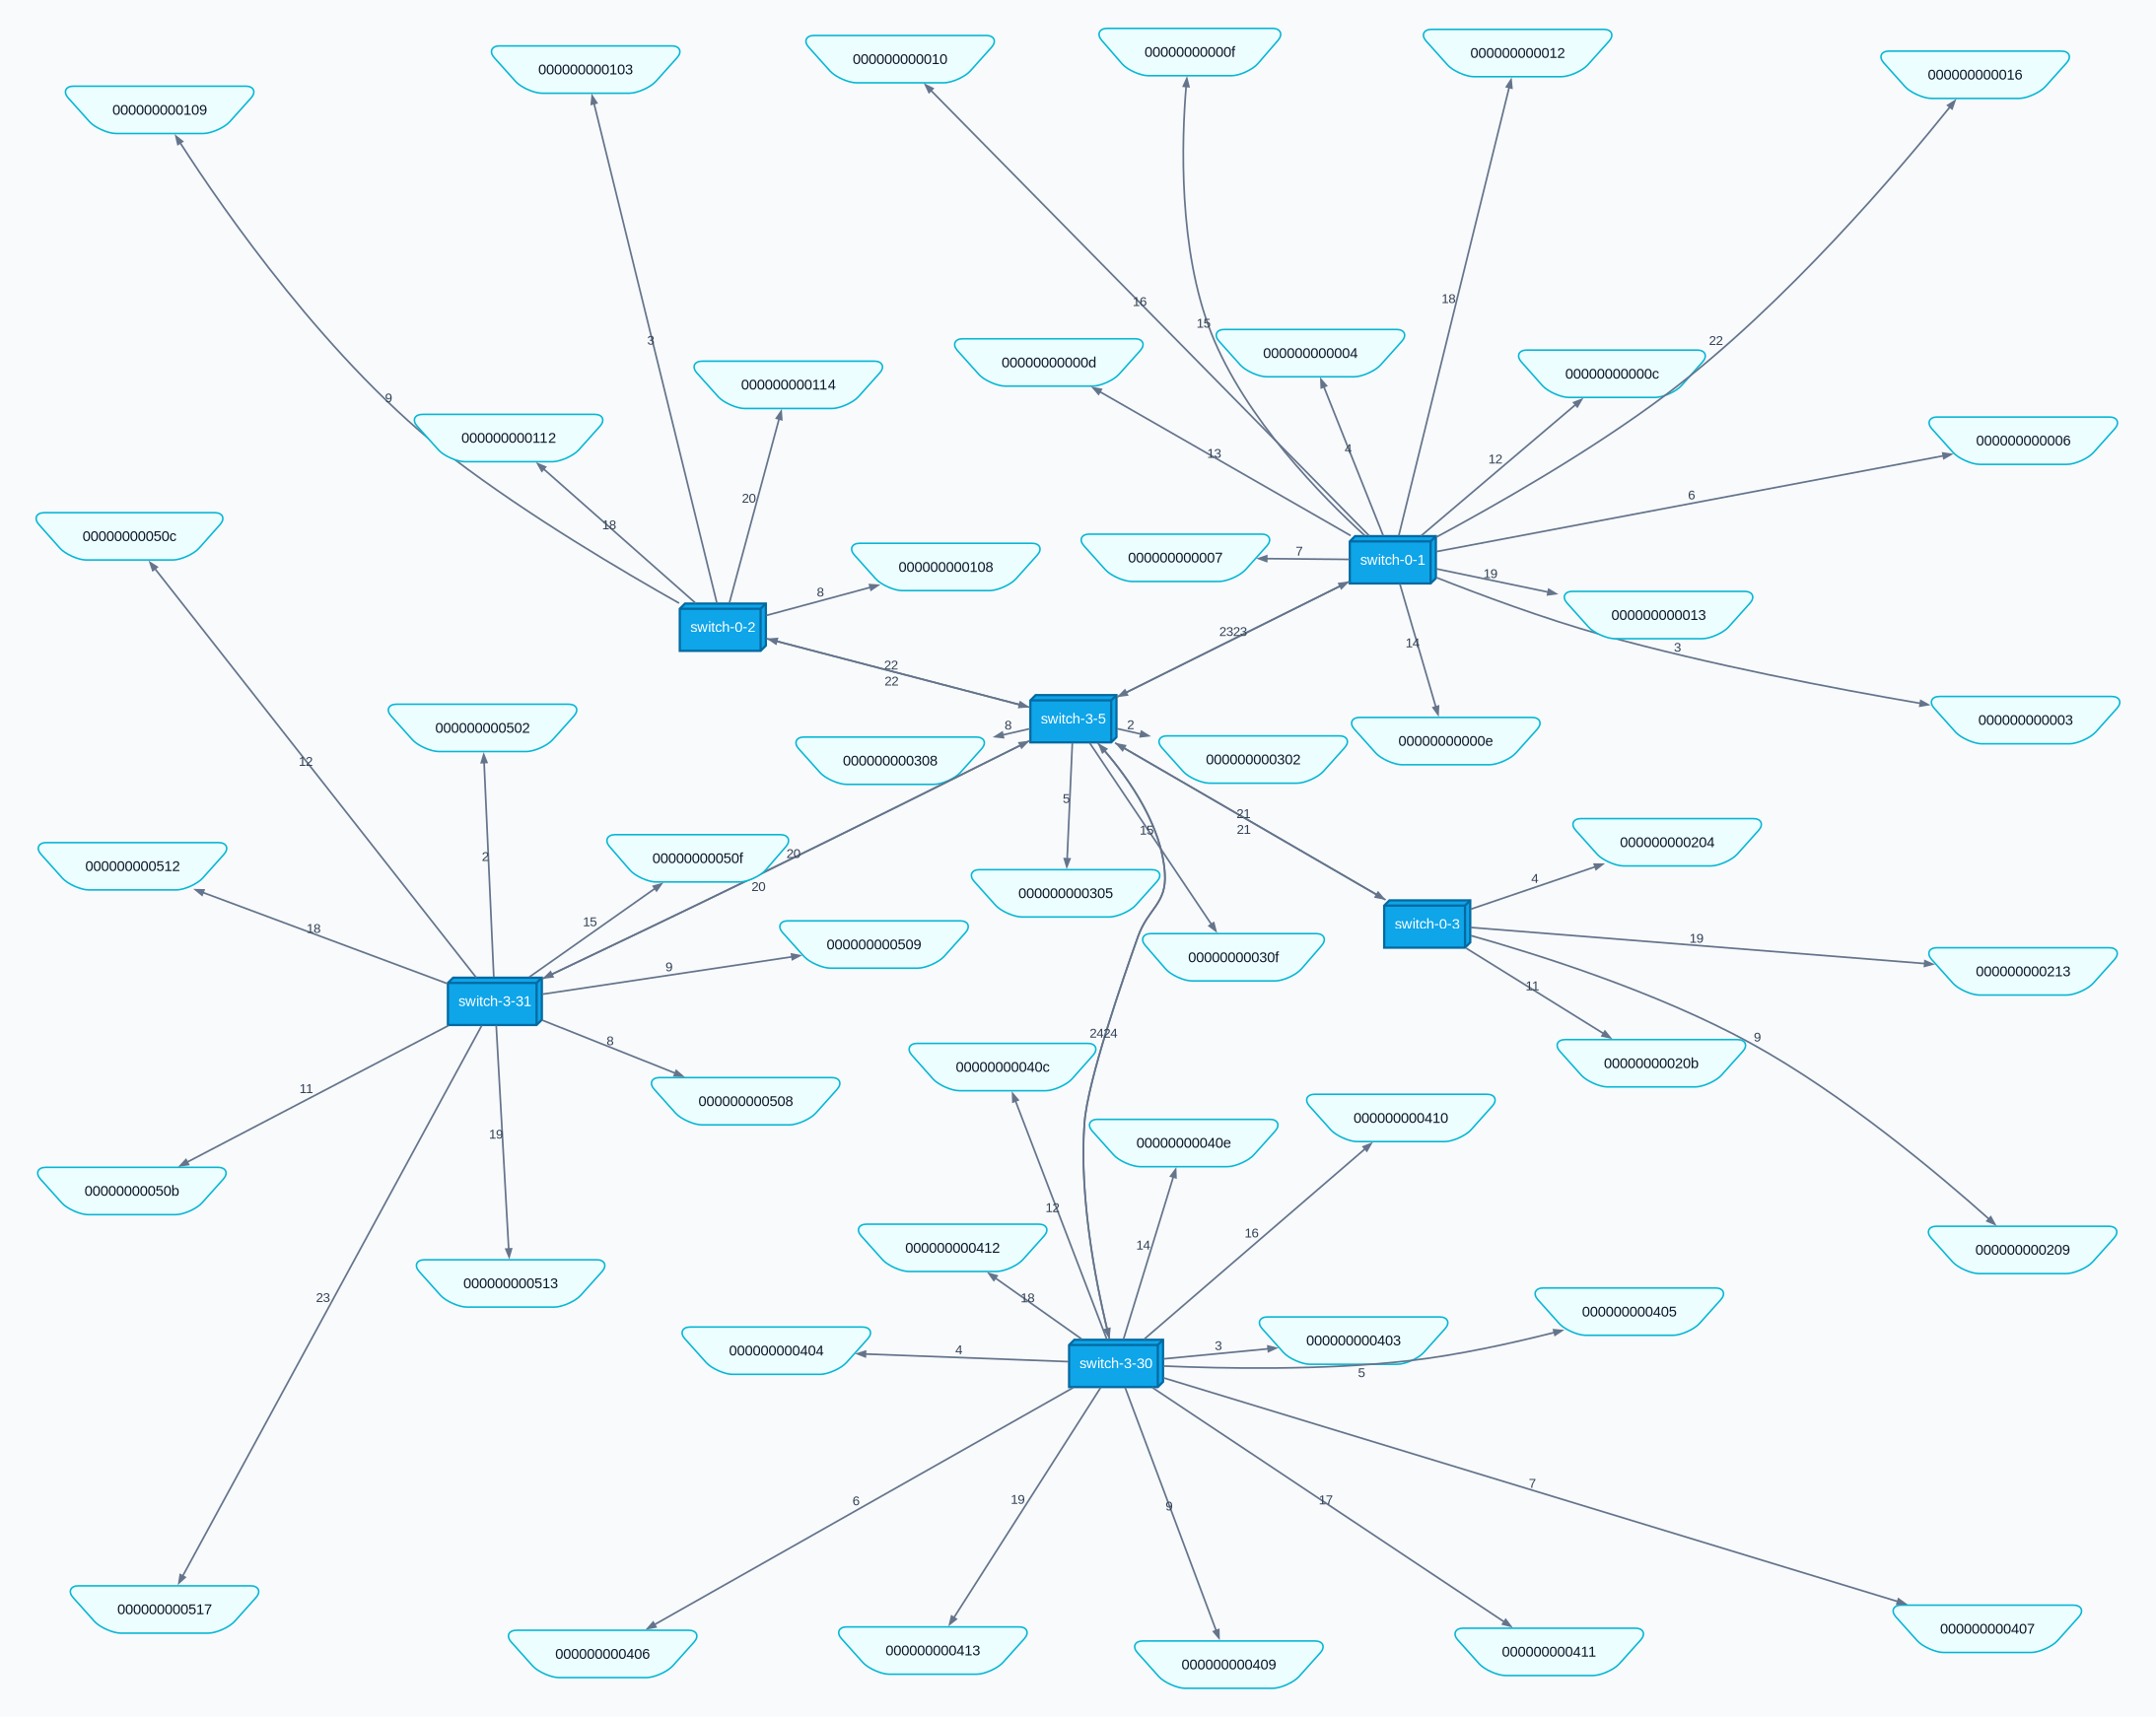
\includegraphics[width=.9\textwidth]{img/simout6star.png}
    \caption{Visualization of the simulated star topology with 6 switches}
    \label{fig:simout6star}
\end{figure}

As in the previous case, it is possible to start the Prolog engine with the generated facts and execute queries to identify 
the inferred topology, which should correspond exactly to the simulated one, with switch-3-5 identified as a core
switch and the other switches identified as access switches. \\

\begin{lstlisting}
# Starting the Prolog engine with simulated facts
% peshmind serve --kbpool kbpool
# Query to identify core switches
% peshmind query "internalswitchn(X)"
# Output:
&{internalswitchn [switch-3-5]}
# Query to identify access switches
% peshmind query "edgeswitchn(X)"
# Output:
&{edgeswitchn [switch-0-1]}
&{edgeswitchn [switch-0-2]}
&{edgeswitchn [switch-0-3]}
&{edgeswitchn [switch-3-30]}
&{edgeswitchn [switch-3-31]}
# Access switches and their connection ports
% peshmind query "edgeswitchpn(X,N)"
# Output:
&{edgeswitchpn [switch-0-1 23]}
&{edgeswitchpn [switch-0-2 22]}
&{edgeswitchpn [switch-0-3 21]}
&{edgeswitchpn [switch-3-30 24]}
&{edgeswitchpn [switch-3-31 20]}
\end{lstlisting}

As can be seen, the inferred topology corresponds exactly to the simulated one, with switch-3-5 identified as a core
switch and the other switches identified as access switches, with interconnection ports correctly highlighted. \\
To visualize the inferred topology, it is possible to generate a DOT file using the \texttt{dot} command and convert it to PNG.
The result is shown in figure \ref{fig:inferred6star}. \\

\begin{lstlisting}[language=bash]
# DOT file generation from inferred topology
peshmind dot > inferred_topology6star.dot
fdp -Tpng inferred_topology6star.dot -o inferred_topology6star.png
\end{lstlisting}

\begin{figure}[ht]
    \centering
    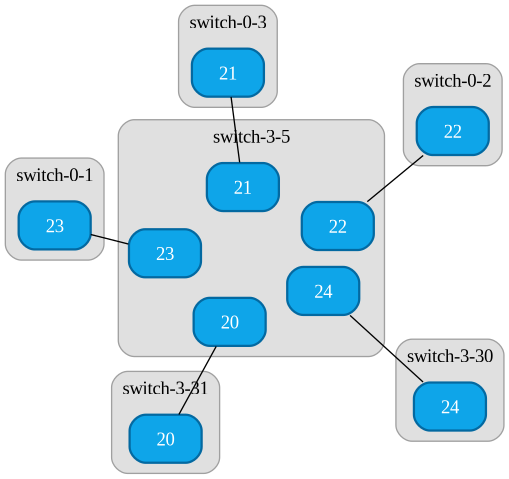
\includegraphics[width=.5\textwidth]{img/inferred6star.png}
    \caption{Visualization of the inferred star topology with 6 switches}
    \label{fig:inferred6star}
\end{figure}

\subsection{Simulation of an Unlisted Switch}

The simulator allows specifying unlisted switches (ghost switches) using the \texttt{ghost="true"} attribute in DOT file
nodes. For example, in the \texttt{topology4ghost.dot} file shown below, privsw-0-1g is a ghost switch. When
the simulator processes this object, it generates Prolog facts without declaring it as a switch, allowing verification that the
inference system can correctly identify the presence of the ghost switch based only on information
from other switches. \\

\begin{lstlisting}[language=DOT]
    digraph dsgraph {
	node [label="\N"];
	"privsw-0-1g" [ghost = true, ports = 24, mac = "004000000001"];
	"privsw-0-2";
	"privsw-3-5";
	"privsw-3-30";
	"privsw-0-1g" -> "privsw-0-2" [port = 24]; 
	"privsw-0-2" -> "privsw-0-1g" [port = 24];
	"privsw-0-1g" -> "privsw-3-5" [port = 23];
	"privsw-3-5" -> "privsw-0-1g" [port = 23];
	"privsw-3-5" -> "privsw-3-30" [port = 24];
	"privsw-3-30" -> "privsw-3-5" [port = 24];
}
\end{lstlisting}

By simulating this topology and starting the Prolog engine, 
it is possible to execute queries to identify the presence
of the ghost switch. For example, the query \texttt{ghostn(X,Y)} 
returns pairs of directly connected switches
that see the same MAC on interconnection ports, 
indicating the presence of a ghost switch between them. \\

\begin{lstlisting}[language=bash]
# Topology simulation with ghost switch
% peshmind simulate --config peshmind.json -d simout4ghost.dot -o kbpool -s topology4ghost.dot --sim-generate-percentage 30
# Starting the Prolog engine with simulated facts
% peshmind serve --kbpool kbpool
# Query to identify ghost switches
% peshmind query "ghostn(X,Y)"
# Output:
&{ghostn [privsw-0-2 privsw-3-5]}
\end{lstlisting}

Also in this case, the inferred topology can be
visualized graphically, as shown in figure \ref{fig:inferred4ghost}, using the \texttt{dot} command, 
and should highlight the presence of the ghost switch 
privsw-0-1g as an intermediate node between privsw-0-2 and
privsw-3-5. \\

\begin{figure}[ht]
    \centering
    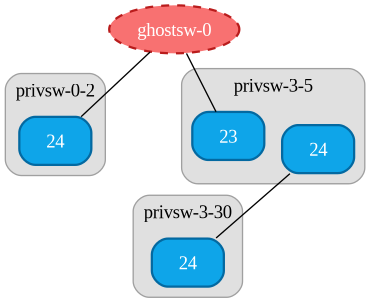
\includegraphics[width=.5\textwidth]{img/inferred4ghost.png}
    \caption{Visualization of the inferred topology with ghost switch}
    \label{fig:inferred4ghost}
\end{figure}

\subsection{Analysis of a Case with Real Data}

As a final example, an analysis of a real
network composed of 6 switches was performed, with data collected through
the \texttt{update} command and loaded into the Prolog engine. 
The switch configuration was defined in the
\texttt{peshmind.json} file shown below. \\

\begin{lstlisting}[language=json]
{
	"debug": true,
	"endpoint": "http://localhost:3030/pengine",
	"switches": {
		"privsw-0-1": {
			"name": "privsw-0-1",
			"mac": "e4..",
			"description": "",
			"ip": "10...",
			"Username": "admin",
			"Password": "ask",
			"model": "HP-Aruba",
			"port": 24,
			"extraports": [],
			"data": ""
		},
		"privsw-0-2": {
			"name": "privsw-0-2",
			"mac": "00..",
			"description": "",
			"ip": "10...",
			"Username": "admin",
			"Password": "ask",
			"model": "HP-Aruba",
			"port": 24,
			"extraports": [],
			"data": ""
		},
		"privsw-200-1": {
			"name": "privsw-200-1",
			"mac": "00..",
			"description": "",
			"ip": "10...",
			"Username": "admin",
			"Password": "ask",
			"model": "HP-Aruba",
			"port": 24,
			"extraports": [],
			"data": ""
		},
		"privsw-200-2": {
			"name": "privsw-200-2",
			"mac": "00..",
			"description": "",
			"ip": "10...",
			"Username": "admin",
			"Password": "ask",
			"model": "HP-Aruba",
			"port": 24,
			"extraports": [],
			"data": ""
		},
		"privsw-2-1": {
			"name": "privsw-2-1",
			"mac": "00..",
			"description": "",
			"ip": "10...",
			"Username": "admin",
			"Password": "ask",
			"model": "HP-Aruba",
			"port": 24,
			"extraports": [],
			"data": ""
		},
		"privsw-3-5": {
			"name": "privsw-3-5",
			"mac": "00..",
			"description": "",
			"ip": "10...",
			"Username": "admin",
			"Password": "ask",
			"model": "HP-Aruba-Press",
			"port": 24,
			"extraports": [],
			"data": ""
		},
		"privsw-3-30": {
			"name": "privsw-3-30",
			"mac": "e00..",
			"description": "",
			"ip": "10...",
			"Username": "admin",
			"Password": "ask",
			"model": "HP-Aruba",
			"port": 24,
			"extraports": [],
			"data": ""
		}
	}
}
\end{lstlisting}

Unlike simulation cases, in this scenario
no information about the network topology is provided,
but only access credentials to switches
to retrieve MAC tables. \\

\begin{lstlisting}[language=bash]
# Updating real switch data
% peshmind update --switch all
# Output:
Updating switch: privsw-0-1
....
# Starting the Prolog engine with real facts
% peshmind serve --kbpool kbpool
\end{lstlisting}

Data collected from real switches may be 
incomplete or noisy, with missing or
contradictory information. Despite this, the inference engine
manages to correctly identify the network topology
and highlight any anomalies or unlisted switches. \\
The inference result can be visualized
graphically, as shown in figure \ref{fig:inferredreal}, using the \texttt{dot} command. \\
\begin{lstlisting}[language=bash]
# DOT file generation from inferred topology
peshmind dot > inferred_real.dot
dot -Tpng inferred_real.dot -o inferred_real.png
\end{lstlisting}    

\begin{figure}[h]
    \centering
    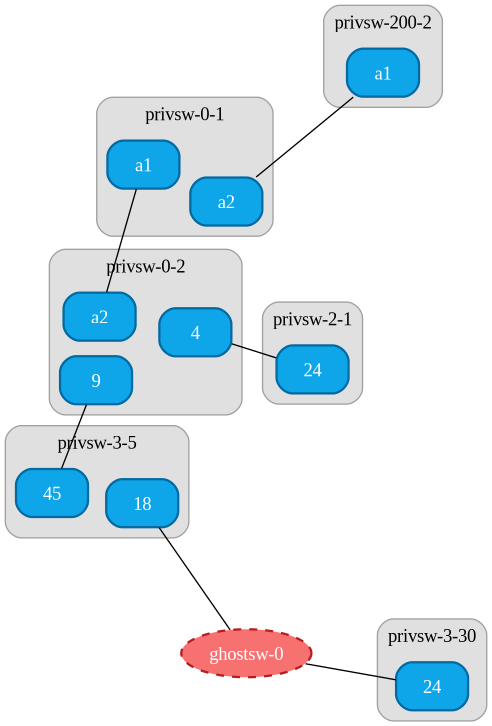
\includegraphics[width=.6\textwidth]{img/inferredreal.png}
    \caption{Visualization of the topology inferred from real data}
    \label{fig:inferredreal}
\end{figure}

The ghost switch detected between privsw-3-5 and privsw-3-30
indicates the presence of an unlisted device that
interconnects these two switches. Indeed, in the real 
network, there is a core switch that was intentionally not 
included in the configuration, but which is 
correctly identified as a ghost switch thanks
to information collected from access switches. \\

\section{Limitations and Future Developments}

\subsection{Current Limitations}

\begin{itemize}
    \item Limited support for switch models, each model needs a specific template
    \item Requires SSH/console access to switches
    \item Does not explicitly handle multiple VLANs
\end{itemize}

\subsection{Possible Future Developments}

\begin{enumerate}
    \item \textbf{More Exhaustive Queries}
    \begin{itemize}
        \item Add templates for a greater number of switch models
        \item SNMP support as an alternative to SSH
    \end{itemize}
    
    \item \textbf{VLAN Analysis}
    \begin{itemize}
        \item Infer VLAN configurations
        \item Identify VLAN configuration errors
    \end{itemize}
    
    \item \textbf{Web Interface}
    \begin{itemize}
        \item Dashboard for interactive visualization
        \item Graphical topology editor
        \item Real-time monitoring
    \end{itemize}
    
    \item \textbf{Integration}
    \begin{itemize}
        \item Export to NetBox, LibreNMS
        \item REST API for integration
        \item Webhooks for change notifications
    \end{itemize}
\end{enumerate}

\section{Conclusions}

peshmind represents an innovative approach to automatic network topology discovery, combining Go's efficiency with Prolog's logical inference power. The system has proven effective in automatically identifying:

\begin{itemize}
    \item Physical connections between switches
    \item Undocumented switches (ghost switches)
    \item Switch classification (core vs. access)
    \item Network topology anomalies
\end{itemize}

The combination of an intuitive CLI interface with a logical reasoning engine provides network administrators with a powerful tool to understand, document, and validate their network infrastructures.

The project is released under the Apache 2.0 license, promoting adoption and contribution from the open source community.

\section{Bibliography and References}

\begin{itemize}
    \item SWI-Prolog Documentation: \url{https://www.swi-prolog.org/}
    \item Pengines Library: \url{https://www.swi-prolog.org/pldoc/man?section=pengines}
    \item Cobra CLI Framework: \url{https://github.com/spf13/cobra}
    \item Graphviz Documentation: \url{https://graphviz.org/}
    \item Go Programming Language: \url{https://golang.org/}
\end{itemize}

\appendix

\end{document}
